% !TeX spellcheck = en_US
\documentclass[french]{yLectureNote}

\title{Mécanique}
\subtitle{Mécanique du point}
\author{Paulhenry Saux}
\date{\today}
\yLanguage{Français}

\professor{S.Deheuvels}%sebastien.deveuhels.irap.omp.eu

\usepackage{graphicx}%----pour mettre des images
\usepackage[utf8]{inputenc}%---encodage
\usepackage{geometry}%---pour modifier les tailles et mettre a4paper
%\usepackage{awesomebox}%---pour les boites d'exercices, de pbq et de croquis ---d\'esactiv\'e pour les TP de PC
\usepackage{tikz}%---pour deiffner + d\'ependance de chemfig
\usepackage{tkz-tab}
\usepackage{chemfig}%---pour deiffner formules chimiques
\usepackage{chemformula}%---pour les formules chimiques en \'equation : \ch{...}
\usepackage{tabularx}%---pour dimensionner automatiquement les tableaux avec variable X
\usepackage{awesomebox}%---Pour les boites info, danger et autres
\usepackage{menukeys}%---Pour deiffner les touches de Calculatrice
\usepackage{fancyhdr}%---pour les en-t\^ete personnalis\'ees
\usepackage{blindtext}%---pour les liens
\usepackage{hyperref}%---pour les liens (\`a mettre en dernier)
\usepackage{caption}%---pour la francisation de la l\'egende table vers Tableau
\usepackage{pifont}
\usepackage{array}%---pour les tableaux
\usepackage{lipsum}
\usepackage{yFlatTable}
\usepackage{multicol}
\usepackage{cancel}
\usepackage{xcolor}
\newcommand\Ccancel[2][black]{\renewcommand\CancelColor{\color{#1}}\cancel{#2}}
\newcommand{\Lim}[1]{\lim\limits_{\substack{#1}}\:}
\renewcommand{\vec}{\overrightarrow}
\newcommand{\norm}[1]{||\vec{#1}||}
\newcommand{\dd}[0]{\mathrm{d}}
\newcommand{\ddp}[0]{\partial}
%\DeclareMathOperator\arctanh{arctanh}
\DeclareMathOperator\grad{grad}
\begin{document}

%\titleOne
\setcounter{chapter}{7}
	\chapter{Puissance, travail et énergie}
% \section{Énergie}
% \subsection{Différentes sources d'énergie}
% \begin{itemize}
%  \item Énergie électrique, thermique, lumineuse, nucléaire, chimique
%  \item Énergie cinétique, potentielle, mécanique
% \end{itemize}
% \subsection{Approche historique}
% Débat autour de la quantité conservée : $m\vec{v}$ ou $m\norm{v}^2$ ?
%
% Expérience d'Émimilie de Chatelet
%
% Lagrange : Théorème des forces vives (Théorème de l'énergie cinétique)
%
% \begin{theorem}[Théorème des forces vives]
% \[\Delta E_c = \sum_i w(\vec{F_i})\]
% \end{theorem}
%
% Prise en compte des échanges de chaleur (Thermodynamique)
% \subsection{Définition}
% C'est une quantité scalaire qui quantifie la capacité d'un système à modifier un état, et donc à produire un travail qui entraîne :
% \begin{itemize}
%  \item un mouvement
%  \item du rayonnement
%  \item de la chaleur
% \end{itemize}
% On la mesure en Joules  = 1$kg\cdot m^2\cdot s^{-2}$ (SI), en électron-Volt = $1.6\cdot10^{-19}$ J. C'est l'énergie acquise par une différence de potentiel. Il y a aussi le $kWh = 1000\times 3600 J = 3.6MJ$. Enfin, la calorie
\section{Puissance d'une force}
\subsection{Définition}
\begin{theorem}[Définition d'une force]
Soit une force $\vec{F}$ appliquée à un système $M$ se déplaçant à une vitesse $\vec{v}_{M/R}$. La puissance de $\vec{F}$ est donnée par
$P = \vec{F}\cdot\vec{v}$ et s'exprime en Watt ($kg\cdot m^2\cdot s^{-3}$. Elle dépend du référentiel d'étude.
\end{theorem}
\begin{multicols}{2}
La puissance est positive si $\theta \in[\frac{-\pi}{2},\frac{\pi}{2}]$. On dit que la force est motrice au temps où la puissance est calculée.\marginCritical{La puissance est instantanée. Cela signifie qu'au cours d'un mouvement, la force peut \^etre motrice ou résistante. C'est le cas de la force de rappel du ressort pendant une oscillation.}

La puissance est négative si $\theta \in[\frac{\pi}{2},\frac{3\pi}{2}]$. On dit que la force est résistante au temps où la puissance est calculée.

\columnbreak
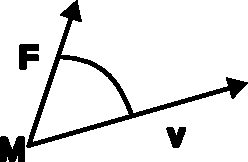
\includegraphics{path6}
\end{multicols}
\subsection{Théorème de la puissance cinétique}
\begin{theorem}[Théorème de la puissance cinétique]
La dérivée temporelle de l'énergie cinétique vaut la somme des puissances des forces exercées sur le système.
\[\dot{E_c} = \sum_i P(\vec{F_i})\]
\end{theorem}
\begin{myproof}
Il découle du PFD, appliqué au système ramené à un point $M$
\begin{flalign*}
m\vec{a} &= \sum_i \vec{F_i}\\
(m\vec{a} &= \sum_i \vec{F_i})\cdot\vec{v}\\
m\vec{a}\cdot\vec{v} &= \sum_i \vec{F_i} \cdot\vec{v}\\
\frac{1}{2}m\frac{\mathrm{d}\norm{v}^2}{\mathrm{d}t} &= \sum_i \vec{F_i} \cdot\vec{v}\\
\frac{\mathrm{d}}{\mathrm{d}t}(\frac{1}{2}m\norm{v}^2) &= \sum_i \vec{F_i} \cdot\vec{v}\\
\frac{\mathrm{d}}{\mathrm{d}t}(E_c) &= \sum_i \vec{F_i} \cdot\vec{v}\\
\end{flalign*}
\end{myproof}
On perd l'information sur les forces qui sont perpendiculaires au déplacement mais on gagne en simplicité. Un raisonnement énergétique peut simplifier les choses.
\subsubsection{Exemple sur le pendule}
On fait un bilan des forces :
\[
 \left\{\begin{matrix}
\vec{T} =& -T\vec{e_{\rho}}\\
\vec{P} =& -mg\sin\varphi \vec{e_{\varphi}}
\end{matrix}\right.\]

$P(\vec{T}) = \vec{T}\cdot\vec{v} = (-T\vec{e_{\rho}})\cdot(l\dot{\varphi}\vec{e_{\varphi}}) = 0$ car $\vec{T}\perp \vec{v}$\marginTips{On rappelle que l'expression de la vitesse en coordonnées polaire avec un rayon constant est $\rho\dot{\varphi}\vec{e_{\varphi}}$}

$P(\vec{P}) = \vec{P}\cdot\vec{v} = -mgl\sin(\varphi)\times \dot{\varphi}$.

On applique le TPC :
\begin{flalign*}
\dot{E_c} &= P(\vec{P}) + P(\vec{T})\\
\frac{1}{2}m\frac{\mathrm{d}}{\mathrm{d}t}l^2\dot{\varphi}^2 &= -mgl\sin(\varphi)\times \dot{\varphi}\\
\frac{1}{2}\frac{\mathrm{d}}{\mathrm{d}t}l\dot{\varphi} &= -g\sin(\varphi)\\
l\ddot{\varphi} + g\sin(\varphi) &=0
\end{flalign*}

En faisant l'approximation des petits angles, on retrouve l'EQD trouvée avec l'analyse classique (PFD).
\section{Travail et Théorème de l'énergie cinétique}
\subsection{Travail d'une force}
Soit un système se déplaçant de A vers B suivant un chemin $C(AB)$. On veut connaitre le travail d'une force $\vec{F}$ lors de ce déplacement. On décompose le chemin en déplacements élémentaires $\mathrm{d}\vec{r}$ et on introduit le travail élémentaire $\delta W$\marginInfo{On l'écrit $\delta W$ et non $\mathrm{d} W$, car généralement, ce n'est pas la différentielle d'une fonction $W$ car cela signifirait que $\in_A^B\mathrm{d}f = f(B)-F(A)$ et donc que $W$ ne dépend que des points et non du chemin.}, avec $\delta W = \vec{F} \cdot \mathrm{d}\vec{r}$ car $\vec{F}$ est considérée comme constante sur ce petit déplacement.

On a alors le travail de la forc F sur le chemin $C(AB)$
\begin{equation}
 W_{C(AB)} (\vec{F}) = \int_{C(AB)}\delta W = \int_{C(AB)} \vec{F} \cdot \mathrm{d}\vec{r}
\end{equation}
On appelle circulation du vecteur $\vec{F}$ sur le chemin $C(AB)$ la quantité précédente.

\subsubsection{Propriétés}
\begin{itemize}
 \item On peut séparer le chemin en morceau, puis sommer les travaux
 \item Si on parcourt le chemin dans l'autre sens, le travail sera opposé.
 \item Généralement, la circulation dépend du chemin emprunté entre les 2 points.
 \item Si $W > 0$, la force est dite motrice, dans le cas contraire elle est négative, si $W=0$, la force ne travaille pas.
\end{itemize}
\subsubsection{Déplacement élémentaire}
On a $\vec{v} = \frac{\mathrm{d}\vec{r}}{\mathrm{d}t} \iff \mathrm{d}\vec{r} = \vec{v}\times \mathrm{d}t$.

En cartésien à 3D : $\mathrm{d}\vec{r} = \mathrm{d}x\vec{e_x} + \mathrm{d}y\vec{e_y} + \mathrm{d}z\vec{e_z}$

En cylindrique : $\mathrm{d}\rho\vec{e_{\rho}} + \rho\mathrm{d}\varphi\vec{e_{\varphi}} + \mathrm{d}z\vec{e_z}$.
\subsection{Calcul du travail d'une force}
\subsubsection{Forces $\perp$ au mouvement}
On a $W_{C(AB)} (\vec{F}) = \int_{C(AB)} \vec{F} \cdot \mathrm{d}\vec{r} = \int_{C(AB)} 0$. Elle ne fournit aucun travail.
\subsubsection{Cas d'une force constante}
On a $W_{C(AB)} (\vec{F}) = \int_{C(AB)} \mathrm{d}\vec{r} = \vec{F} \cdot\int_{C(AB)} \mathrm{d}\vec{r} = \vec{F} \cdot \vec{AB}$. En effet, la somme de tous les petits déplacement élémentaires donne $\vec{AB}$.
\checkInfo{Exemple du poids}{
On dit que le poids est constant : $W_{C(AB)} (\vec{P}) = \vec{F} \cdot \vec{AB} = -mg(z_b-z_a)$. On peut aussi faire
\begin{flalign*}
W_{C(AB)} (\vec{P}) &= \int \vec{P} \cdot \mathrm{d}\vec{r}\\
&= \int \vec{P} \cdot (\mathrm{d}x\vec{e_x} + \mathrm{d}y\vec{e_y} + \mathrm{d}z\vec{e_z})\\
&= \int -mg \mathrm{d}\vec{z}\\
&= -mg(z_b-z_a)
\end{flalign*}
}
\subsubsection{Forces non constantes}
Force de rappel du ressort : Dans un déplacement après $l_0$, on a $W_{C(AB)} (\vec{F_r}) = \int_{C(AB)} \vec{F_r} \cdot \mathrm{d}\vec{r} = \int\vec{F_r} \cdot (\mathrm{d}x\vec{e_x} + \mathrm{d}y\vec{e_y} + \mathrm{d}z\vec{e_z}) = \int\vec{F_r} \cdot \mathrm{d}x\vec{e_x} =  \int^{x_b}_{x_a}-kx \mathrm{d}x = -k[\frac{x^2}{2}]^{x_b}_{x_a} = -\frac{1}{2}k(x_b^2-x_a^2)$

Si $|x_b| > |x_a|$, la force est résistante.
% \checkInfo{Exemple sur 3 trajectoires}{
% On considère une force $\vec{F} = a(y^2x\vec{e_x}+x^2y\vec{e_y})$
% 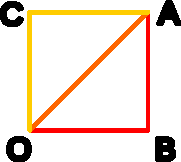
\includegraphics{path1}
% }
% On cherche $W_1 = W_{C_1}$, $W_2 = W_{C_2}$, $W_3 = W_{C_3}$
\subsection{Théorème de l'énergie cinétique}
\begin{theorem}[Énoncé]
\[\Delta_{AB} E_c = \sum_i W_{C,AB}(\vec{F_i})\]
\end{theorem}
\begin{myproof}[À partir du TPC]
On utilise aussi le fait que $\vec{v}\times\mathrm{d}t = \mathrm{d}r$ car $\frac{\mathrm{d}\vec{r}}{\mathrm{d}t}$.
\begin{flalign*}
\frac{\mathrm{d}E_C}{\mathrm{d}t} &= \sum_i P(\vec{F_i})\\
\int_{t_a}^{t_b}\frac{\mathrm{d}E_C}{\mathrm{d}t}\mathrm{d}t &=\int_{t_a}^{t_b} \sum_i (\vec{F_i})\cdot \vec{v} \times \mathrm{d}t\\
E_c(B)-E_c(A) &= \sum_i \int \vec{F_i}\cdot \mathrm{d}\vec{r}\\
&= \sum_i \int \delta W\\
&= \sum_i W_{C,AB}(\vec{F_i})
\end{flalign*}
\end{myproof}
\checkInfo{Exemple d'application}{On étudie une particule dans un champ électrique constant. (exercice 5.1) On veut connaître la valeur de $\vec{v_d}$. On a donc, avec $\vec{F_e} = eE_0\vec{e_x}$ la force électrostatique.
\begin{flalign*}
 E_c(d) - E_c(0) &= \sum_i W_{C,AB}(\vec{F_i})\\
  E_c(d) - E_c(0) &= W_{C,OA}(\vec{F_e})\\
  &= \int_{0,d} \vec{F_e}\cdot \mathrm{d}r\\
  &= \int_{0,d} qE_0\vec{e_x}\cdot \mathrm{d}x\vec{e_x}\\
  &= \int_{0,d} qE_0\mathrm{d}x\\
  &= qE_0d\\
\end{flalign*}
On peut maintenant multiplier par $\frac{2}{m}$ et obtenir $v_d$.}
\section{Énergie potentielle et forces conservatives}
\subsection{Notion de forces conservatives}
\subsubsection{Notion de différentielle}
Pour une fonction $f$ qui est $C^1$, on peut définir $\dd f(a) = f(a+\dd x) - f(a)$.

La dérivée est $f'(a) = \Lim{\dd\to 0} \frac{f(a+\dd x)-f(a)}{\dd x}$.

On a donc $\dd f(a) = f'(a)\dd x \iff f'(a) = \frac{\dd f(a)}{\dd x}$. On peut le généraliser au cas de fonctions de plusieurs variables $f(x,y,z)$ et obtenir des dérivées partielles pour chaque variables.

$\dd f = \frac{\partial f}{\partial x}\dd x + \frac{\partial f}{\partial y}\dd y + \frac{\partial f}{\partial z}\dd z$.
\subsubsection{Force conservative}
\begin{definition}[Définition 1]
Une force $\vec{F}$ est dite conservative s'il existe une fonction $u(\vec{r})$ de l'espace tel que le travail élémentaire $\delta W(\vec{F}) = \vec{F}\cdot \dd \vec{r}$ soit égal à $\delta W = -\dd u$.
\end{definition}
\begin{definition}[Définition 2]
Une force est conservative $\iff$ le travail de $\vec{F}$ dans le déplacement de A vers B ne dépend pas du chemin pris.
\end{definition}
\begin{myproof}
Si $\vec{F}$ est conservative, alors $\exists u(\vec{r})$ telle que $\delta W = -\dd u$. On a donc
\begin{flalign*}
W(\vec{F}) &= \int \delta W(\vec{F})\\
&= -\int \dd u\\
&= -[u(B)-u(A)]
\end{flalign*}
Cette dernière expression ne dépend pas du chemin.
\end{myproof}
\begin{definition}[Définition 3]
$\vec{F}$ est conservative $\iff$ le travail sur tout chemin fermé est nul (le point de départ = point d'arrivée).

On a alors $W(\vec{F}) = \oint \delta W$.
\end{definition}
\begin{myproof}
Soit 2 points A et B et 2 chemins. Le chemin $C_1-C_2$ est fermé, donc $W(\vec{F}) = 0 \iff W_{C_1} (\vec{F}) - W_{C_2}(\vec{F}) = 0 \iff W_{C_2}(\vec{F}) = W_{C_1}(\vec{F})$.
\end{myproof}
\subsection{Énergie potentielle}
\begin{definition}[Énergie potentielle]
Si une force $\vec{F}$ est conservative, il existe une fonction $u$ telle que $\delta W(\vec{F}) = -\dd u$. On appelle $u$ énergie potentielle, notée $E_{P_F}$.
\end{definition}

Ainsi, $W(\vec{F}) = \int \delta W = -\int dE_p = -E_p(B)-E_p(A)$. La variation d'énergie potentielle sur $AB$ vaut l'opposé du travail, autrement dit\marginTips{On peut dire aussi $\Delta E_p$ vaut le travail qu'un utilisateur doit fournit pour amener le système du point A au point B.} :\[\Delta_{AB} E_p = -W_{C,AB}(\vec{F})\]

\warningInfo{Conséquence}{L'énergie potentielle est définit à une constante près. Il faut donc se fixer un point de référence où elle est nulle.}
\subsubsection{Méthode}
Une façon de calculer $E_p$ est d'écrire $\delta W = -\dd E_p \iff \vec{F}\cdot \dd \vec{r} = -\dd E_p$. Il faut ensuite intégrer.
\subsubsection{Exemple du poids}
$\vec{P} = -mg\vec{e_z}$. On veut \begin{flalign*}
\delta W(\vec{P}) &= - \dd E_p \\
\vec{P}\cdot \dd \vec{R} &= -\dd E_p\\
(-mg\vec{e_z}\cdot(\dd x\vec{e_x}+\dd y\vec{e_y}+\dd z\vec{e_z}) &= -\dd E_p\\
-mg\dd z &= -\dd E_p\\
\frac{\dd E_p}{\dd z} &= mg\\
E_p = mgz + CST
\end{flalign*}
On choisit $E_p = 0$ pour $z=0$, dans ce cas la constante vaut $0$ et $E_p = mgz$. Le signe de l'expression dépend de l'axe.
\subsection{Opérateur gradient}
Soit une fonction $u$ de $\mathbb{R}^3 \to \mathbb{R}$. On introduit un vecteur $\grad(u)$ tel que $\dd u = \grad(u)\cdot \dd \vec{r}\label{grad}$. En cartésien, $\dd u = \frac{\partial u}{\partial x}\dd x + \frac{\partial u}{\partial y}\dd y + \frac{\partial u}{\partial z}\dd z$ et selon \eqref{grad}, $\dd u = \grad_x(u) \dd x + \grad_y(u) \dd y + \grad_z(u)\dd z$.

On obtient le vecteur gradient en cartésien :\marginInfo{L'expression du gradient dépend du système de coordonnées dans lequel on se trouve}
\[\grad(u) =  \begin{pmatrix}
\frac{\partial u}{\partial x} \\
 \frac{\partial u}{\partial y}\\
 \frac{\partial u}{\partial z}
\end{pmatrix}\]

\subsubsection{Propriétés}
\begin{itemize}
 \item Il est linéaire
 \item Il est dirigé dans le sens des $u$ croissants, c'est à dire pour maximiser l'augmentation de $u$.
 \item Il est orthogonal aux équipotentielles de $u$, surfaces sur lesquelles $u$ est constant.
\end{itemize}
\begin{myproof}
\begin{flalign*}
\dd u &= \grad(u)\cdot \dd\vec{r}\\
&= \norm{\grad(u)} \times \norm{\dd r} \times \cos(\theta)
\end{flalign*}
Si $\dd \vec{r}$ est dans la direction et le sens de $\grad(u)$, alors $\dd u$ est maximal, car $\theta = 0$ et $\cos = 1$

Si on se déplace orthogonalement à $\grad(u)$, $\dd u = \norm{\grad(u)} \times \norm{\dd u} \times 0$. Le grandient est orthogonal aux équipotentielles de $u$, surfaces sur lesquelles $u$ est constant.
\end{myproof}
\subsection{Calcul de $E_p$ avec le gradient}
Pour une force conservative, on a $\delta W = \vec{F}\cdot \dd \vec{r} = -\dd E_p$ et $\dd E_p = \grad(E_p)\cdot \dd \vec{r}$, donc $\vec{F}\cdot \dd \vec{r} = -\grad(E_p)\cdot\dd \vec{r}$. On obtient que \[\vec{F} = -\grad(E_p)\].
\begin{definition}[Définition 4 d'une force conservative]
Une force $\vec{F}$ est conservative $\iff$ il existe une fonction $E_p$ telle que $\vec{F} = -\grad(E_p)$. On dit que $\vec{F}$ dérive d'une énergie potentielle.
\end{definition}
Cette définition est utile pour calculer une énergie potentielle.

\checkInfo{Exemple du poids}{
Avec un axe orienté vers le haut. $\vec{P} = -mg\vec{e_z}$. On cherche une fonction $E_p$ telle que $\vec{P} = -\grad(E_p)$. On a donc :

$-\frac{\partial E_p}{\partial x} = 0 \Rightarrow E_p$ ne dépend pas de $x$

$-\frac{\partial E_p}{\partial y} = 0 \Rightarrow E_p$ ne dépend pas de $y$

$-\frac{\partial E_p}{\partial z} = -mg \Rightarrow \frac{\dd E_p}{\dd z} = mg \Rightarrow E_p = mgz + Cst$.}

\subsection{Calcul de $E_p$ pour des forces conservative}
\subsubsection{Force de rappel du ressort}
$\vec{F_r} = -kx\vec{e_x}$. On cherche $E_p$ telle que $\vec{F_r} = -\grad(E_p)$. Elle ne dépend ni de $y$ ni de $z$. On a alors $-kx = -\frac{\dd E_p}{\dd x} \iff E_p = \frac{1}{2}kx^2 + Cst$. On choisit souvent l'énergie potentielle nulle à l'équilibre, ici on prend $E_p=0$ pour $x=0$, car on a choisit de mettre l'origine à la longueur à vide.
\subsubsection{Force de gravitation}
$\vec{F_g} = -\frac{GMm}{r^2}\vec{e_r}$ C'est valable dans la base sphérique. On a donc $\vec{F_g} = -\grad(E_p)$, donc : $-GMm\frac{1}{r^2} = -\frac{\dd E_p}{\dd r} \iff E_p = -GmM\frac{1}{r} - Cst$. On se donne $E_p\to 0$ quand $r\to \infty$, donc il faut que la constante soit nulle.
\subsubsection{Force électrostatique}
$\vec{F_e} = -\frac{qq_0}{4\pi\varepsilon_0\times r^2}$. C'est valable dans la base sphérique où la force ne dépend que du vecteur $\vec{e_r}$, on a donc : $\vec{F_e} = -\grad(E_p)$, donc : $-\frac{1}{4\pi\varepsilon_0}\times\frac{qq_0}{r^2} = -\frac{\dd E_p}{\dd r}\iff E_p = -\frac{1}{4\pi\varepsilon_0}\times\frac{qq_0}{r}+Cst$.

On choisi que $E_p\to0$ quand $r\to \infty$, donc la constante est nulle.
\section{Énergie mécanique}
\begin{definition}[Définition]
C'est l'énergie cinétique plus la somme des toutes les énergies potentielles des forces conservatives.
\end{definition}
\subsection{Théorème de l'énergie mécanique}
\begin{theorem}[]
La variation de l'énergie mécanique correspond à la somme des travaux des forces non conservatives, qui dissipent de l'énergie, comme les frottements. \[\Delta_{AB} = \sum_i W_{C,AB}(\vec{F_{NC}})\]
\end{theorem}
\begin{myproof}[À partir du TEC]
\begin{flalign*}
\Delta E_c &= \sum_i W(\vec{F_i})\\
&=\sum_i W(\vec{F_{c,i}}) + \sum_i W(\vec{F_{nc,i}})\\
\Delta E_c - \sum_i W(\vec{F_{c,i}}) &= \sum_i W(\vec{F_{nc,i}})\\
\Delta E_c - (-\Delta E_p) &= \sum_i W(\vec{F_{nc,i}})\\
\Delta E_c +\Delta E_p &= \sum_i W(\vec{F_{nc,i}})\\
\Delta E_m &= \sum_i W(\vec{F_{nc,i}})\\
\end{flalign*}
\end{myproof}
% Exemple : Force de frottement en $-\alpha \vec{v}$ : Travail sur un chemin fermé strictement négatif.

En l'absence de forces non conservatives, l'énergie mécanique se conserve.\marginTips{Si les forces conservatives en présence ont des $E_p$ connues, on utilise plut\^ot ce théorème.}
\subsection{Théorème de la puissance mécanique}
\begin{theorem}[TPM]
\[\frac{\dd E_m}{\dd t} =\sum_j P(\vec{F_{NC,j}})\]
\end{theorem}
\begin{myproof}[À partir du TPC]
\begin{flalign*}
\frac{\dd E_c}{\dd t} &= \sum_k P(\vec{F_c}) + \sum P(\vec{F_{NC}})\\
&= \sum \vec{F_C}\cdot \vec{v}+\sum P(\vec{F_{NC}})\\
&= \sum \vec{F_C}\cdot \frac{\dd \vec{r}}{\dd t}+\sum P(\vec{F_{NC}})\\
&= \sum \delta W(\vec{F_C} \frac{1}{\dd t}+\sum P(\vec{F_{NC}})\\
&= \sum \frac{-\dd E_p}{\dd t}+\sum P(\vec{F_{NC}})\\
&\Rightarrow \frac{\dd E_m}{\dd t} =\sum_j P(\vec{F_{NC,j}})
\end{flalign*}
\end{myproof}
\section{Interprétation graphique de l'énergie potentielle}
On s'interesse à des systèmes dont le mouvement possède un seul degré de liberté\marginTips{Un seul paramètre décrit le mouvement (cas d'un mouvement rectiligne par exemple, mouvement circulaire à rayon constant)} et conservatif. On considère $E_p$ la somme de toutes les énergies potentielles. On note $\vec{F}$ la résultante des forces. $E_p$ correspond donc à l'énergie potentielle associée à $\vec{F}$.

Il y a un seul degré de liberté : $\vec{F}(x) = F(x)\vec{e_x}$. On peut écrire $\vec{F} = -\grad(E_p)\Rightarrow F(x) = -\frac{\dd E_p}{\dd x}$.

On peut alors interpréter le graphique $E_p$ en fonction de $x$.

\subsubsection{Position d'équilibre}
L'accélération est nulle, donc $\vec{F} = \vec{0} \iff -\frac{\dd E_p}{\dd x} =0$, donc les positions d'équilibre correspondent aux points où la courbe $E_p(x)$ admet une tangente horizontale, aux extremum locaux par exemple.
\subsubsection{Signe de la dérivée}
Si $\frac{\dd E_p}{\dd x}>0, F(x)<0$ (courbe croissante)

Si $\frac{\dd E_p}{\dd x}<0, F(x)>0$

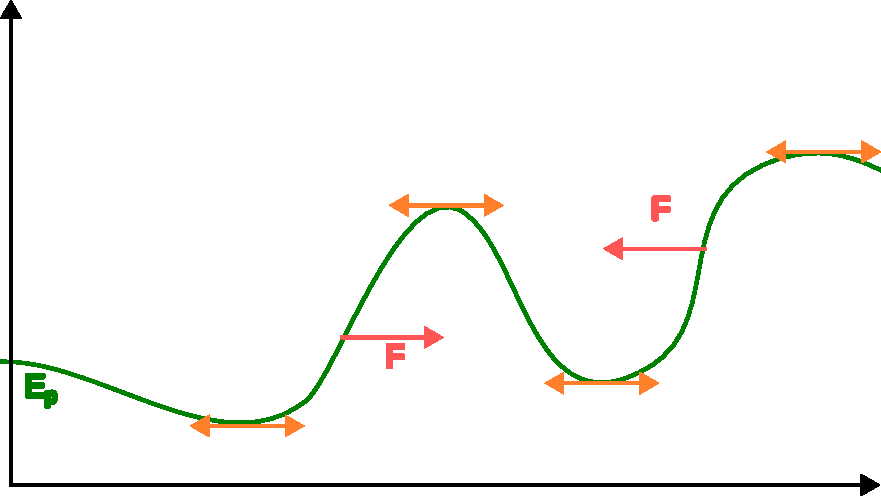
\includegraphics[scale=0.5]{graph}
\subsection{Stabilité des positions d'équilibre}
\begin{definition}
Une position d'équilibre est site stable si elle revient à cette position après une petite perturbation car les forces en présence tendent à l'y ramener. Dans le cas contraire, elle est instable.
\end{definition}
\subsubsection{Condition pour qu'une position d'équilibre soit table}
Soit $x_0$ une positon d'équilibre, $F(x) = 0 \iff -\frac{\dd E_p}{\dd x} = 0$\marginCritical{Il s'agit bien de la dérivée en fonction de $x$ en non la dérivée temporelle}

Pour qu'une position soit stable, il faut que $F(x_0+\dd x)<0$ quand $x>0$ ou $F(x_0+\dd x)>0$ quand $x<0$

On réécrit la première égalité :
\begin{flalign*}
 \frac{F(x_0+\dd x)-F(x_0)}{\dd x} &< 0\\
 \frac{\dd F}{\dd x}(x_0) &< 0 \iff -\frac{\dd^2 E_p}{\dd x^2} <0\\
 \frac{\dd^2 E_p}{\dd x^2}&>0
\end{flalign*}
Il faut donc que la courbe soit convexe en $x_0$

En ajoutant l'information de l'$E_m$, on peut conna\^itre l'évolution du système.

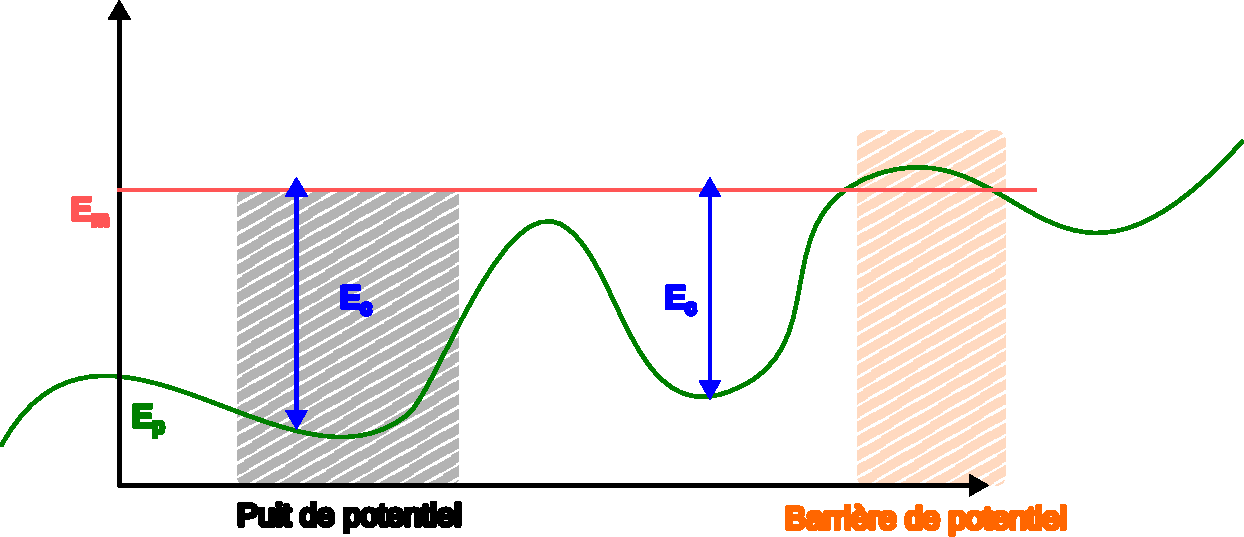
\includegraphics[scale=0.5]{rect5}

\end{document}

